\chapter{\texorpdfstring{\acrlong*{acc:ea}}{}}

Optimization. What better word would describe the ultimate goal of all the people, our civilization, and maybe even the Universe. With a bit of exaggeration, optimization is the cause of all the ramifications we can see around. Because what else are Physic laws than minimization processes, our pursuit of knowledge and self improvement than maximization of self-worth, industrial revolutions than minimization of human labour, maximization of goods production and standard of living at the same time. In my opinion, optimization is the reason what drives us forward, makes us better, and guides our decisions.

One of the most extraordinary optimization processes is, without a doubt, evolution. Evolution is nothing less than Nature way of improvement species to better adapt to their environment. The father of evolution is undoubtedly Charles, who the first come up with an idea of evolution in his work \enquote{On the origin of species: A facsimile of the first edition} \citep{darwin1964origin}. According the him, the individuals that better adapted to the environment have higher potential to reproduce and pass their genetic material --- including the predisposition to survive in the environment --- to their offsprings. Sometimes referred as \enquote{Survival of the fittest}.

This exact ideas inspired scientists and formed the field of \acrfull{acc:ea}\index{evolutionary algorithm}\footnote{I will refer to all the population-based algorithms in this work as \acrlong*{acc:ea}. These includes, among others, \acrlong*{acc:ga}, \acrlong*{acc:ea}, and \acrlong*{acc:pso}.}.
\acrshort{acc:ea} are stochastic, population-based optimization algorithms inspired by biological evolution. In general, a set of individuals called population compete with each other for a place in the next generation. Each individual represent one possible solution of the problem in hand. Quality of the individual is proportional to the quality of solution it represents. This quality is usually expressed using fitness (or sometimes called objective) function. As with natural evolution, the probability of survival is proportional the solution quality -- the better the solution is, the higher the probability of survival \citep{IntroductionToEA}. In the \acrshort{acc:ea}, the process of producing new generation is usually called selection.

Evolution is not only about survival, but also about reproduction. \acrlong*{acc:ea} took inspiration here as well and uses specials operators for each generation -- usually called evolution operators or variation operators\index{variation operator}. As the name suggests, these operators make sure the population explores new solutions. The two most common operators are crossover and mutation. During crossover\index{crossover}, individuals from the current population (usually called parents) produces new individuals (usually called offsprings) by combining their genetic information. In some way, crossover mimic reproduction in Nature, during which the \acrshort{acc:dna} of offspring is by majority determined by its parents \acrshort{acc:dna}. Mutation\index{mutation}, on the other hand, causes random small alteration of the individual genetic material and is able to introduce novel patterns that did not previously occur in the population \citep{HowToSolveItModernHeuristics}.

In general, \acrshort{acc:ea} repeat steps above until sufficiently good solution is found, or until maximum number of generations is reached. The general pseudocode of the \acrshort{acc:ea} algorithm is in Algorithm \ref{alg:SEA}. I will present more accurate implementations of various algorithms thorough this chapter.

\begin{algorithm}
    \SetAlgoLined
    \KwResult{evolved population}
    initialize population\;
    \Repeat{termination criteria met}{
        reproduction\;
        mutation\;
        evaluate population\;
        selection\;
    }
    \caption{General Evolution Algorithm}
    \label{alg:SEA}
\end{algorithm}




%%%%%%%%%%%%%%%%%%%
%%               %%
%%  TERMINOLOGY  %%
%%               %%
%%%%%%%%%%%%%%%%%%%
\section{Terminology}

In this section, I will introduce necessary terminology that I am going to use thorough this work. I took most of the terminology from \citet{IntroductionToEA}.

\defterm{Problem} is the function we want to solve. It can be both satisfactory as well optimization problem.

\defterm{Genotype}\index{genotype} is encoding of the solution. It is equivalent of the \acrshort{acc:dna} -- it compress all the data needed to produce solution.

\defterm{Gene} is one part of the genotype. It may be one bit if the genotype is encoded as binary string or scalar, if the genotype is vector. 

\defterm{Representation or genotype space} is the space of genotype.

\defterm{Phenotype}\index{phenotype} is the solution built from genotype. Genotype and phenotype can be equivalent -- for example real function optimization problem may have as a genotype vector of real numbers, that represent one of the solution. Generally, however, genotype and phenotype can be different \citep{GeneticAlgorithmEssentials}.

\defterm{Search space} is the space of phenotype.

\defterm{Objective function} is the function the algorithm optimize. For previous example of real function optimization, the function itself can be the objective function. I will denote objective function $\objectivefn$.

\defterm{Fitness function}\index{fitness function} is the measure of quality of the solution. Note that the domain of the function is the search space. Unlike the objective function, the fitness function should guide the algorithm during the optimization. It can use the objective function directly, but other options are possible as well. For example, if the goal is to maximize objective function $\objectivefn(x)$, but the algorithm is written such that it minimize the fitness function, one may specify the fitness function as $\fitnessfn(x)=\frac{1}{\objectivefn(x)}$. I will denote fitness function $\fitnessfn$.

\defterm{Evaluation} is the process of obtaining fitness value for the genotype.

\defterm{Individual} is genotype with it's fitness value. I will denote individual by $\individual$.

\defterm{Fitness value} of individual is it's evaluation. 

\defterm{Population} is multiset of individuals -- it is possible to have same genotype in the population multiple time. However, I will still distinguish different individuals with the same genotype. I will denote the whole population as $\population$.

\defterm{Initialization} is the process of creating the first population.

\defterm{Exploitation} is the effort to use knowledge from the history in order to maximize the expected outcome \citep{SelfAdaptiveFeaturesInRealParameterEvolutionaryAlgorithms}.

\defterm{Exploration} is the effort to discover new rules about the problem in hand, although the expected outcome does not need to be the best possible. In general, the biggest problem in \acrshort{acc:ea} is the right balance between exploitation and exploration. Putting too much emphasis may cause to get stuck in the local minima, whereas putting too much focus on the exploration may cause, that the algorithm never converge. Note that \acrshort{acc:ea} is not the only field suffering from this, but for example Reinforcement Learning deals with the same problems \citep{ExplorationExploitationDilemaRL}. 

\defterm{Evolution operators} are individual steps performed each iteration.

\defterm{Selection}\index{selection} is evolution operator that picks up individuals from the current population to the next one. The selection should take into account fitness of each individual in the population and pick them proportionally. Selection therefore implements the \enquote{Survival of the fittest} law. From the mathematical point of view, selection task is to move the population into more promising area of the search space and possibly to reduce variance of the population \citep{SelfAdaptiveFeaturesInRealParameterEvolutionaryAlgorithms}. In other word, selection is exploitation step in the algorithm.

\defterm{Crossover}\index{crossover} is evolution operator, that combines some individuals (usually called \textbf{parents}) in order to create one or more new individuals (usually called \textbf{offsprings}). Offsprings are usually combination of their parents, similarly to how \acrshort{acc:dna} of the child is combination of \acrshort{acc:dna} of her parents.

\defterm{Mutation}\index{mutation} is evolution operator, that modify one individual. Mutation can be based on randomness (for example replacement of value in genotype by different value) or specialized for the problem in hand. This time the example can be \acrlong{acc:tsp}, where one possible mutation operator can \enquote{untwist} ways that cross each other. This mutation is in fact local optimization technique, as the  mutated way is shorter than the previous one \citep{TSPArticle}.

\defterm{Variation operators}\index{variation operator} are operators, that change the variation of the population, but not the mean. Variation operators are the exploration steps in the algorithm and should balance the exploitation strength of the selection. Both crossover and mutation are variation operators \citep{SelfAdaptiveFeaturesInRealParameterEvolutionaryAlgorithms}.

\defterm{Memetic operator} is operator, that uses local optimization in every iteration. Alternatively, \enquote{memetic algorithms uses local optimizer to every solution before evaluation} \citep{HowToSolveItModernHeuristics}. One of such example is the \acrlong{acc:tsp} problem mentioned earlier. Another example is the problem of searching for weights in \acrshort{acc:ann}, where one step of backpropagation algorithm is performed as part of the mutation.




%%%%%%%%%%%%%%%%%%%%%%%%%%
%%                      %%
%%  GENETIC ALGORITHMS  %%
%%                      %%
%%%%%%%%%%%%%%%%%%%%%%%%%%
\section{\texorpdfstring{\acrlong*{acc:ga}}{}}

\acrfull{acc:ga}\index{genetic algorithm} are probably the simplest \acrfull{acc:ea} out there and as their father is usually considered \citefullauthor{HollandGA}. In the \acrshort{acc:ga}, individual are binary string of length $n$, formally
$$ \individual \in \left\{0,1\right\}^{n} $$

Fitness function maps genotype into real values
$$ \fitnessfn:\left\{0,1\right\}^{n}\rightarrow\mathbb{R} $$

The typical crossover operator is \emph{one point crossover}\index{crossover \acrshort*{acc:ga}!one--point}. This type of crossover require two parents and produces two offsprings. As the first step, the algorithm uniformly sample random integer $s$ in the range $\left[ 1, n-1 \right]$. The first offspring will receive genetic material up to index $s$ from the first parent, and the rest from the second one. The second offspring is created the same way, except the position of parents is exchanged. Example for $n=10$ is in figure \ref{fig:gaonepointcrossover}. In order not to modify all the individuals in the population, only $p_c\in\left[0,1\right]$ percent of individuals undergo the crossover and the children replace their parents \citep{IntroductionToEA}.

\begin{figure}
    \begin{subfigure}[b]{0.4\textwidth}
        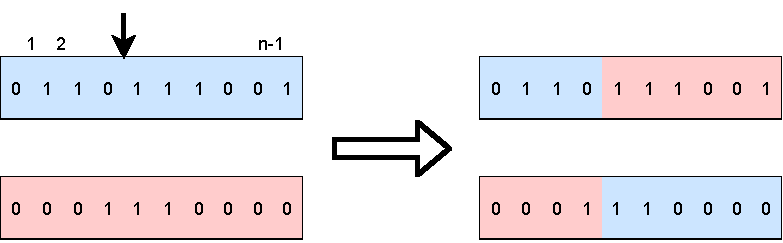
\includegraphics[width=\textwidth]{img/master_onepointcrossover.pdf}
        \caption{One point crossover}
        \label{fig:gaonepointcrossover}
    \end{subfigure}
    \hfill
    \begin{subfigure}[b]{0.4\textwidth}
        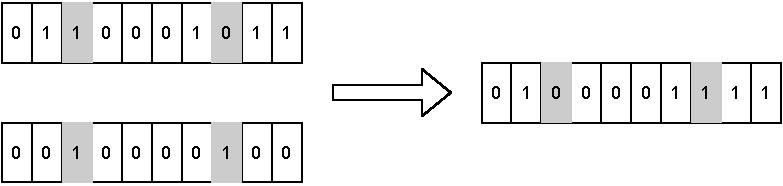
\includegraphics[width=\textwidth]{img/master_bitflipmutation.pdf}
        \caption{Bit--flip mutation}
        \label{fig:bitflipmutation}
    \end{subfigure}
    \caption{Genetic algorithm operators}
\end{figure}

The mutation\index{mutation \acrshort*{acc:ga}} operator for \acrshort{acc:ga} is in most cases bit--flip mutation\index{mutation \acrshort*{acc:ga}!bit--flip}. During this mutation, each gene in the genotype is mutated with probability $p_m$. One example of mutation is in figure \ref{fig:bitflipmutation}. Mutation has two objectives -- it makes sure the algorithm is not trapped in local optima, and it sustains genetic disparity in the population. As a side effect, mutation serves as minor search operator \citep{IntroToGA}.

The difference between crossover and mutation is such that crossover is rather \enquote{search} exploitation technique. It combines individuals from current population and exploit them to find possibly better individuals. Mutation, on the other hand, is more local search technique and based on the probability $p_b$ it search over the whole representation space.

Finally, the selection stage takes place. There are various selection techniques and in this particular case, I will use tournament selection\index{selection!tournament}. During tournament selection, fitness values of two random individuals are compared and the better individual is copied into the new population. This repeats as many times, as specified number of individuals form a new population.

For cases where the size of the new population equals to the size of the old one, there is high probability that the same individual will be in the following population multiple times. Nevertheless, because of crossover and mutation operators that does not matter, because variation operators keep divergence in the population.

The pseudocode of simple genetic algorithm described above is depict in algorithm \ref{alg:SGA}. The population if firstly randomly initialized and then undergo crossover, mutation, evaluation, and selection operators in the loop. Finally, evolved population is returned from the algorithm.

\begin{algorithm}
    \KwIn{$d$ problem dimension, $l$ population size, $g$ generations, $\fitnessfn$, $p_c$, $p_m$}
    \KwResult{evolved population}
    population $\leftarrow$ randomly initialized\;
    \ForEach{$gen$ in $0$..$g$}{
        \ForEach{individual in $0$..$l$}{
            \If(){$rand()<p_c$}{One point crossover with random individual}
            \If(){$rand()<p_m$}{Bit--flip mutation}
        }
        Evaluate population using $\fitnessfn$\;
        population $\leftarrow$ pick up $l$ individuals using tournament\;
    }
    \Return{population}
    \caption{Simple genetic algorithm}
    \label{alg:SGA}
\end{algorithm}

I will refer to algorithm described above as \enquote{Simple Genetic Algorithm}. In reality, scientists come up with various operators, that can improve convergence or can help in specific types of problems. Thorough following paragraphs, I will focus on these techniques, inspired mainly by the book of authors \citet*{IntroToGA}.

%%%%%%%%%%%%%%%%%%%%%%
%%%%  CROSSOVERS  %%%%
%%%%%%%%%%%%%%%%%%%%%%
\subsection{Advanced crossover operators}

Simple genetic algorithm used one point crossover. It is straightforward to extend it into \emph{two point crossover}\index{crossover \acrshort*{acc:ga}!two point} where each genome is split into three parts. Each offspring then receives first and third part of the genome from one parent, and the middle one from the second one. Example of two point crossover is in the picture \ref{fig:gatwopointcrossover}.

\begin{figure}
    \begin{subfigure}[b]{0.4\textwidth}
        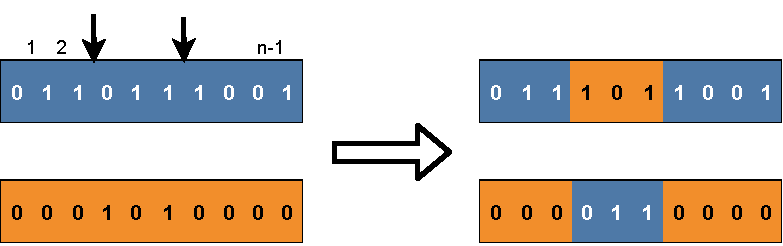
\includegraphics[width=\textwidth]{img/master_twopointcrossover.pdf}
        \caption{Two point crossover}
        \label{fig:gatwopointcrossover}
    \end{subfigure}
    \hfill
    \begin{subfigure}[b]{0.4\textwidth}
        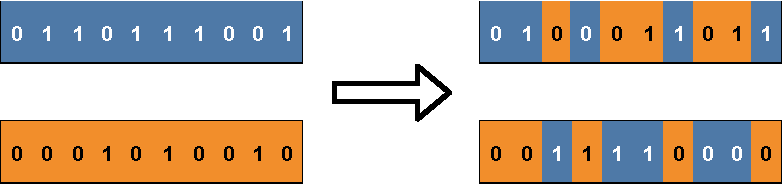
\includegraphics[width=\textwidth]{img/master_uniformcrossover.pdf}
        \caption{Uniform crossover}
        \label{fig:uniformcrossover}
    \end{subfigure}
    \caption{Advanced crossover operators}
\end{figure}

Sometimes, the crossover operator is generalized even more and forms $k$--point crossover. The genotype partitions into $k$ parts and these parts are interleaved in the offsprings. Special case is \emph{uniform crossover}\index{crossover \acrshort*{acc:ga}!uniform} -- the offsprings are constructed in such a way that they are uniform combination if their parents. Each gene in the offspring have equal probability whether it will be received from the first, or second parent. Second offspring will follow the same pattern, except with parents exchanged. Example of uniform crossover is in figure \ref{fig:uniformcrossover}.
% Introduction into GA presents few more types - three parents crossover, crossover with reduced surrogate, and shuffle crossover. These are irrelevant for my implementation, but can be potentially described here.

I have described the crossover operators such that the offsprings replace their parents. That is a common design decision, however one does not need to enforce it and may decide to create offsprings in addition to the parents. To ensure the population does not increase in size, the selection operator can be implemented in a way that specified number of individuals will be picked up.

%%%%%%%%%%%%%%%%%%%%%
%%%%  SELECTION  %%%%
%%%%%%%%%%%%%%%%%%%%%
\subsection{Selection operators}

Selection operator is one of the most important one, as it is the only operator working with fitness values and therefore the operator responsible for exploitation part of the algorithm. Simple genetic algorithm presented in algorithm \ref{alg:SGA} uses tournament selection -- I will analyze another types of selections thorough following paragraphs.

Selection operators are equivalent of Darwin's selection process in nature. It allows to preserve perspective genetic traits and discard the bad ones. That answer to the \enquote{Survival of the fittest} idea. The distinction between good and bad individual is in respect to the fitness function, selection operators therefore favor individuals with better fitness value.

The degree into which operators endorse better individuals is called \emph{selection pressure}\index{selection pressure}. Selection pressure is major indicator of the algorithm and needs to be balanced with other variation operators. Too big selection pressure may cause the algorithm to converge prematurely. Too low selection pressure, on the other hand, may prolong the convergence and the algorithm may need unnecessary steps before convergence.

\emph{Tournament selection}\index{selection!tournament} is one of the most popular selection operators, because it is easy to implement, the absolute values of fitness are not important (rather relative difference to the other individuals is what matter), and can therefore keep the selection pressure constant. Tournament selection can be naturally extend using $k$ parents -- it increase probability for better individuals and thus increase selection pressure of the operator.

Another popular operator is \emph{Roulette Wheel selection}\index{selection!roulette}. In this operator, the probability of selection is equal to the absolute value of the fitness.
$$ P\left[\individual_i\right] = \frac{\fitnessfn(\individual_i)}{\sum_{j=0}^{l}\fitnessfn(\individual_j)} $$
This can be imagined as roulette wheel, where individuals represent sector of a wheel. Size of sector is proportional to the fitness value of the individual. The selection procedure to pick up $n$ individuals simply spin the roulette $n$--times and select the individuals, on which the roulette stopped. Example of roulette wheel selection is in figure \ref{fig:roulettewheelselection}. Selection operators that depends on the absolute values of fitness value are usually called proportional--based selection\index{selection!proportional--based}.

Slightly improvement of roulette wheel selection is \emph{Stochastic Universal Sampling}\index{selection!stochastic universal sampling}. Because roulette wheel selection samples individuals independently, it may select the same individuals more time that would be expected given its proportion to the rest of the population. In the example in figure \ref{fig:roulettewheelselection}, expected draws of individual $p_3$ is one, however, it has been drawn two times. Stochastic Universal Sampling handles this issue by sampling only one number in the range $\left[0,\frac{\sum_i^l\fitnessfn(p_i)}{l} \right]$ and draw each new individual with $\frac{\sum_i^l\fitnessfn(p_i)}{l}$ offset. The stochastic universal sampling is unbiased and the distribution of drawn individuals is closer to the fitness values distribution in comparison to the roulette wheel selection. Example of stochastic universal sampling is in figure \ref{fig:USB}.

\begin{figure}
    \begin{subfigure}[t]{0.47\textwidth}
        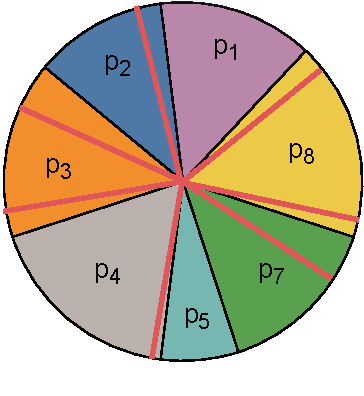
\includegraphics[width=0.8\textwidth]{img/master_roulettewheel.pdf}
        \caption{Roulette wheel selection. Red lines represents sampled individuals.}
        \label{fig:roulettewheelselection}
    \end{subfigure}
    \hfill
    \begin{subfigure}[t]{0.47\textwidth}
        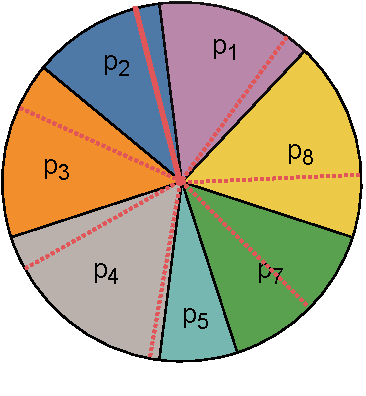
\includegraphics[width=0.8\textwidth]{img/master_stochasticuniversalsampling.pdf}
        \caption{Stochastic universal sampling. Red line represent sampled number and dotted lines are sampled individuals with $\frac{1}{7}$ offset.}
        \label{fig:USB}
    \end{subfigure}
    \caption{Roulette based selections}
\end{figure}

Notice that for both selection operators with higher fitness value the probability of being picked up to the next population increases. These operators are therefore intended for maximization problems. Also, because the fitness value directly affect the size of the circle sector, the fitness function must be positive over the whole domain. It is possible to discard individuals with non positive fitness values, however then the whole selection procedure lose relevance.

One more drawback of both roulette wheel selection and stochastic universal sampling is that the probabilities depends on the absolute values of fitness. Lets look at two cases:
\begin{itemize}
    \item The population fitness values are distributed in the range $\left[ 99,100 \right]]$.
    \item The population fitness values are distributed in the range $\left[ 1, 2\right]$.
\end{itemize}
In both cases, the expected difference of fitness between any two individuals is the same, however, because roulette wheel selection takes into account absolute values of fitness, probability for drawing best individual from the first case is much smaller in comparison to the second case. This effect is usually called \emph{proportional based selection} and it describes situation, where selection probability depends not on the absolute values of fitness function.

Drawback of proportional based selection is that it does not create enough selection pressure when the population has roughly same fitness value. This is problem also to the end of the evolution, because all the individuals are optimized over the generations and have usually very similar fitness value. Note that tournament selection does not suffer by this, as only the relative order between individuals decide about the selection.

One way to eliminate this problem is to rescale fitness to have more desired properties\index{fitness scaling}. One common example is linear scaling into interval $\left[ l,u \right]$ so that individual with $\min\fitnessfn(x_i)=l; \max\fitnessfn(x_i)=u$ and rest of them is scaled linearly between them. 
$$
f_{scale}(\individual)=\frac{\fitnessfn(\individual) - \min\limits_{i}\fitnessfn(\individual_i)}{\max\limits_{i}\fitnessfn(\individual_i)}\cdot(u-l)+l 
$$
Alternatively, logarithmic respectively exponential scale is possible as well, so there will be more emphasis on individuals from the beginning of the sorted sequence, respectively lesser importance of individuals from the end.

Special example of fitness scaling is \emph{rank selection}\index{selection!rank}. To eliminate dependency on the absolute values of fitness function, rank selection assign artificial fitness values to the individuals based on their order in the sorted sequence. One common rank evaluation function is linear -- it assign new fitness values in interval $\left[l,u\right]$ such that best individual has new fitness value $l$, the worst one $u$ and rest of the population is uniformly distributed in this interval (in case of minimization) \citep{razali2011genetic}. Different scaling schemas are possible as well. 

Advantage of rank selection is steady selection pressure and unlike roulette wheel selection can handle negative fitness function. Moreover, is is easy to control selection pressure using interval width, as shown in table \ref{tab:rankselection}. It also does not suffer of outliers -- individuals with very high or low fitness in comparison to the rest of the population. Rank selection can therefore avoid premature convergence, but computation costs can be very costly, because the population needs to be sorted, fitness values reevaluated, and another proportional--based selection operator needs to follow.

\begin{table}
    \centering
    \begin{tabular}{|c c | c c | c c |}
        \hline
        \thead{Fitness\\value} & Rank & 
        \thead{New fitness\\for $\left[1,2\right]$}  & 
        \thead{Selection\\probability\\for $\left[1,2\right]$} &
        \thead{New fitness\\for $\left[1,10\right]$} &
        \thead{Selection\\probability\\for $\left[1,10\right]$} \\
        \hline
        12   & 1   & 2     & $27\%$ & 10    & $38\%$ \\
        7    & 2   & 1.75  & $23\%$ & 7.5   & $29\%$ \\
        1    & 3   & 1.5   & $20\%$ & 5     & $19\%$ \\
        0    & 4   & 1.25  & $17\%$ & 2.5   & $10\%$ \\
        -5   & 5   & 2     & $13\%$ & 1     & $4\%$  \\
        \hline
    \end{tabular}
    \caption{Rank selection pressure}
    \label{tab:rankselection}
\end{table}

Selection operators may use traditional approaches from search algorithms -- for example \emph{simulated annealing}\index{selection!simulated annealing}. Simulated annealing is analogy to metallurgy, where by precise control of heating and cooling of material are improved it's physical and chemical properties. In general it accepts worse solutions as long as the temperature $\tau$ is high enough. The temperature $\tau$ starts high so almost all the solutions are accepted from the beginning, and decrease over time to zero. Decrease is usually exponential: $\tau_g=\tau_0(1-\alpha)^{1+\frac{\beta\cdot g}{G}}$ where $g$ is current generation, $G$ maximum number of generations, $\alpha\in\left[0,1\right]$, $\beta\in\mathbb{R}^+$, and $\tau_0\in\mathbb{R}^+$ are parameters. 

Example of simulated annealing is Boltzmann selection operator. The individual is picked up with probability 
$P=exp\left(-\frac{f_{max} - \fitnessfn(\individual)}{\tau}\right)$
where $f_{max}$ is best fitness in the population and $\tau$ is current temperature (known as Boltzmann probability). Note that Boltzmann selection is once again proportional--based selection operator and may suffer from the same problems as roulette wheel selection.
% TODO Boltzmann selection not implemented

Last selection operator, I would like to discuss, is \emph{elitism}\index{elitism}. For some problems may be beneficial to preserve best individuals from the population. This is especially helpful for problems, where can be optimal solution found using small local steps. Mutation and crossover may destroy the best individual in the population and it may be difficult for the algorithm to found it once again, if it's genetic material have not been propagated yet. 

Elitism mechanism is operator, which makes sure the best individuals remains in the population. It is usually implemented in a way it copies the $k$ best individuals from the population before all other operators, and copy them back afterward. Note that elitism is not really selection operator, but rather insure mechanism not to loose best individuals from the population. Traditional selection operator still needs to be present in order for algorithm to work. 

% TODO schemata are not discussed in the text, it may be worth mention them


%%%%%%%%%%%%%%%%%%%%%%%%%%%%
%%                        %%
%%  EVOLUTION STRATEGIES  %%
%%                        %%
%%%%%%%%%%%%%%%%%%%%%%%%%%%%
\section{\texorpdfstring{\acrlong*{acc:es}}{}}

\acrfull{acc:es} are natural extension of \acrshort{acc:ga} by extension of genotype into real numbers.
$$
\individual \in \mathbb{R}^{n}
$$
Alternatively the relaxed definition allows genotype of arbitrary number of dimension. That may be helpful for problems, which expect particular structure of the solution -- for example image processing filters \citep{WVDF}. Note that using different structure of genotype disallow direct use of some operators, like one and two point crossovers, because the split point may be ambitious. On the other hand, some operators, like uniform crossover, can easily handle multidimensional genotype without much change.

Origin of \acrlong{acc:es} dates to 1970s at Technical University in Technische Universität Berlin, where \citeauthor*{ES-original} presented \acrshort{acc:es} \citep{ES-original}. Originally, \acrshort{acc:ea} has not been used as optimization algorithm for real function, but \enquote{rather as a set of rules for the automatic design and analysis of consecutive experiments with stepwise variable adjustement driving a suitable object/system into the optimal state in spite of enviornmental noise} \citep{EScomprehensiveintroduction}. It turned out thi simple stochastic search technique outperformed traditional--based methods. Although there is no guarantee \acrshort{acc:es} will find optimal solution, they are in most cases able to find near--optimal and sufficiently good enough solution.

This section takes inspiration mainly in the work of \citet*{IntroductionToEA} and \citet*{EScomprehensiveintroduction}.

\acrshort{acc:es} can use same selection and crossover operators as \acrshort{acc:ga}, although it is not recommended \citet{IntroductionToEA}. In general, good crossover operators should
\begin{itemize}
    \item preserve population mean, because crossover operators does not work with a fitness function and therefore should introduce bias in the search space,
    \item slightly increase variance of the population, to balance pressure of selection operators, that usually decrease variance of the population,
    \item\label{enum:espopulationvariance} \snipescondition, so the algorithm effectively search neighborhood solutions,
    \item allow reachability of any solution in the search space.
\end{itemize}
Crossover operators from \acrshort{acc:ga} may fulfil this requirements, however real--coded encoding allows more diverse set of operators. I will describe them a bit later.

\acrshort{acc:ea} also introduced two different selection schemas\index{selection schema}:
\begin{itemize}
    \item $\left(\mu+\lambda\right)$ evolution strategy, also known as \emph{plus schema}.
    \item  $\left(\mu,\lambda\right)$ evolution strategy, also known as \emph{comma schema},
    \item steady--state evolution strategy.
\end{itemize}
Here, the $\mu$ represents number of parents and $\lambda$ number of offsprings. In the first two cases, $\abs{\mu}$ individuals are selected to the next generation, but in the plus schema these individuals are taken from both parents and offsprings. For the comma schema, $\abs{\mu}$ individuals are drawn only from the offsprings and parents are discarded. Obviously, to have at least $\abs{\mu}$ distinct individuals in the next generation, it must hold $\lambda\geq\mu$. For stochastic selection operators, where is possibility to draw same individual multiple times, it may be beneficial to have more offsprings than parents.

Both plus and comma selection schemas generates number of offsprings and resample the whole population for the next generation. Steady--state evolution strategy, on the other hand, generates just one (or a very few) individuals in each generation and try to reintegrate them back into the population. The steps of the algorithm are:
\begin{enumerate}
    \item Generate new individual and evaluate it using fitness function.
    \item\label{enum:steadystateparentpickup} Choose individual from the population, that can be replaced by the new one.
    \item\label{enum:steadystatereplacement} Decide whether the old individual should be replaced.
\end{enumerate}
The step \ref{enum:steadystateparentpickup} is known as the replacement strategy and some of the common variants are to replace the oldest, worst, or random individual. The step \ref{enum:steadystatereplacement} is known as the replacement condition. The most common variant is to replace the old individual only if the new one is better, however is it possible to use simulated annealing as well.
The steady state refer express the idea, that the population undergo only a small change each step \citep{SteadyStateEvolutionStrategy}.

%%%%%%%%%%%%%%%%%%%%%%
%%%%  CROSSOVERS  %%%%
%%%%%%%%%%%%%%%%%%%%%%
\subsection{\texorpdfstring{\acrshort*{acc:ea} crossovers}{}}

Encoding genotype as a vector of real numbers allows, except crossover operators from \acrshort{acc:ga}, additional crossover operators using real numbers. One argument may be exploitation of correlation within the population.

\begin{figure}
    \begin{subfigure}[t]{0.49\textwidth}
        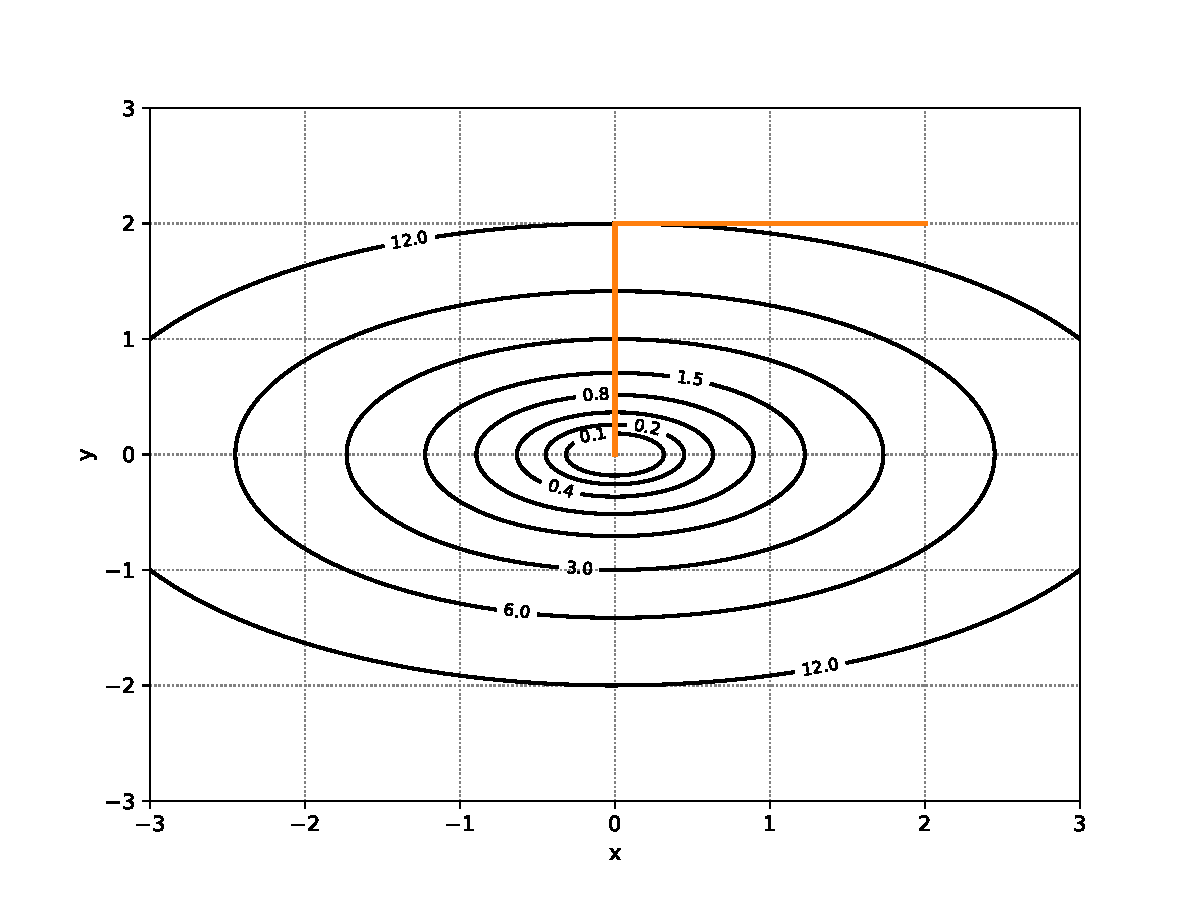
\includegraphics[width=\textwidth]{img/render_separable.pdf}
        \caption{Separable ellipsoid function.}
        \label{fig:separableelipsoid}
    \end{subfigure}
    \hfill
    \begin{subfigure}[t]{0.49\textwidth}
        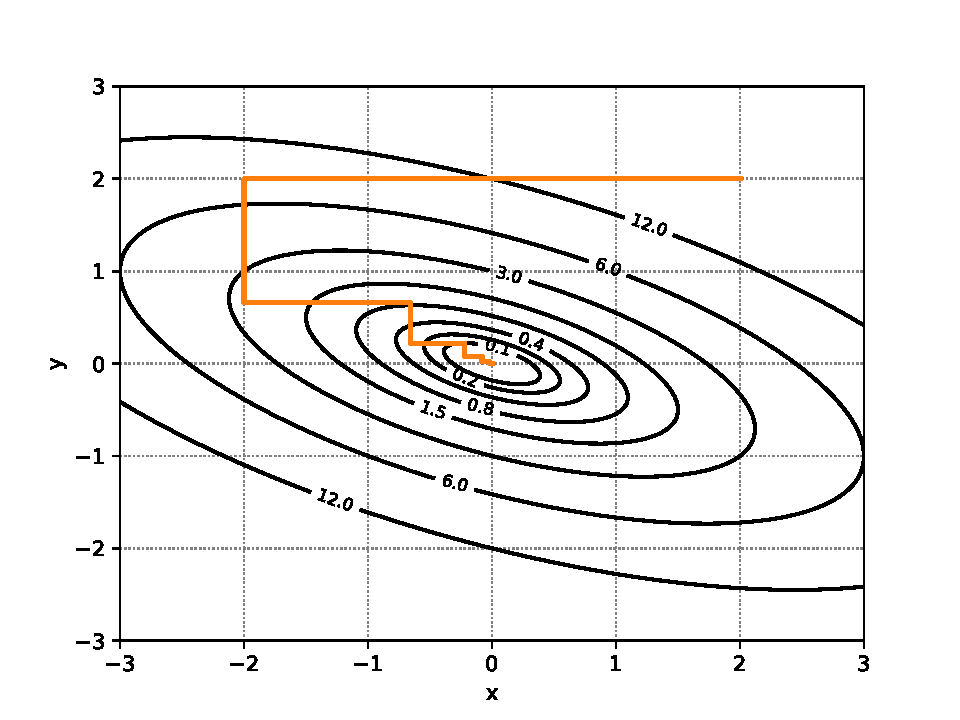
\includegraphics[width=\textwidth]{img/render_nonseparable.pdf}
        \caption{Non--separable ellipsoid function.}
        \label{fig:nonseparableelipsoid}
    \end{subfigure}
    \caption[Difference between separable and non--separable function for optimization]{Difference between separable and non--separable function for optimization. Trajectories of hill climbing algorithm are depict orange.}
    \label{fig:separationfucntions}
\end{figure}

Lets take for example two functions:
\begin{align*}
    f_{sep}(x,y)&=x^2+3y^2 \\
    f_{nosep}(x,y)&=x^2+3y^2+2xy
\end{align*}
These functions are shown in figure \ref{fig:separationfucntions}. Running simple hill climber algorithm \citep{HandbookOfMetaheuristics}, one may get trajectories displayed in the figure by orange color. Notice, that the trajectory of the function $f_{nosep}$ is much longer -- it took $200$ steps to achieve global minimum for the function $f_{sep}$, however up to $400$ steps for the function $f_{nosep}$ (the step size was set equally). The cause of this is that the first function is separable -- it can be written in the form $f_{sep}(x,y)=f(x)+f(y)$. Hill climber algorithm can easily find optimum, because $\min f_{sep}=\min f(x)+\min f(y)$, therefore it can find the optimum for each of the variable independently. That is not true for the function $f_{nosep}$, because it is not separable and using local search technique is not as straightforward. Separable functions are more challenging harder in some sense, the problem \acrshort{acc:ea} should solve efficiently.

Problem of crossover operators from \acrshort{acc:ga} is exactly the same as I just shown you. These operators works on the genes independently, they do not use knowledge about the correlation of the genotype space within the population. It is necessary to use different crossover operators tailored for the \acrshort{acc:ea}.

One of the simplest \acrshort{acc:es} crossover is \emph{arithmetic crossover}\index{crossover \acrshort*{acc:es}!arithmetic}. For parents $\mathbf{p_1}$ and $\mathbf{p_2}$, the offspring $o$ is created using following formula.
$$
\mathbf{o} = \alpha\mathbf{p_1}+\left(1-\alpha\right)\mathbf{p_2}
$$
where $\alpha \sim U(0,1)$ (uniformly distributed variable in interval $\left[0,1\right]$). Is is possible to generate second offspring by setting $\beta=1-\alpha$ and substitute $\beta$ for $\alpha$. This operator uses same $\alpha$ for every dimension of the vector, so it is sometimes called \emph{whole arithmetic crossover}. Easy extension is to use $\boldsymbol{\alpha}=(\alpha_1,\alpha_2,\dots,\alpha_n)$ vector, where $\alpha_i\sim U(0,1)$ and create offspring using similar formula.
$$
\mathbf{o} = \boldsymbol{\alpha}\cdot\mathbf{p_1}+\left(1-\boldsymbol{\alpha}\right)\cdot\mathbf{p_2}
$$
where $\cdot$ is element--wise multiplication of vectors.
Natural extension of the algorithm is to use up to $k$ parents $\mathbf{p_1}, \mathbf{p_2},\dots,\mathbf{p_k}$ and create offspring by their linear combination.
$$
\mathbf{o} = 
\boldsymbol{\alpha}_1\cdot\mathbf{p_1}+
\boldsymbol{\alpha}_2\cdot\mathbf{p_2}+
\cdots +
\boldsymbol{\alpha}_k\cdot\mathbf{p_k}
$$
where $\sum_{i=1}^{k}\boldsymbol{\alpha}_i=\boldsymbol{1}$.
% TODO make sure the implementation checks

Arithmetic crossover is just a linear combination of it's parent, it does not satisfy condition on page \pageref{enum:espopulationvariance} to \enquote{\snipescondition}. Authors \citeauthor*{BlendCrossoverOriginal} address this issue in \emph{blend crossover}\index{crossover \acrshort*{acc:es}!blend} operator. For parents $\mathbf{x}$ and $\mathbf{y}$, the genes of offspring $\mathbf{o}$ is generated randomly from uniform distribution specified by it's parents.
$$
o_i = U\left( 
    x_i - \alpha \left( y_i - x_i \right),
    y_i + \alpha \left( y_i - x_i \right)
\right)
$$
Here, the $\alpha$ is user specified parameter and algorithms is sometimes called \acrshort{acc:blx}--$\alpha$ crossover. Example of \acrshort{acc:blx} is in the figure \ref{fig:blendcrossoverexample}.
% TODO not implemented

\begin{figure}
    \begin{subfigure}[t]{0.45\textwidth}
        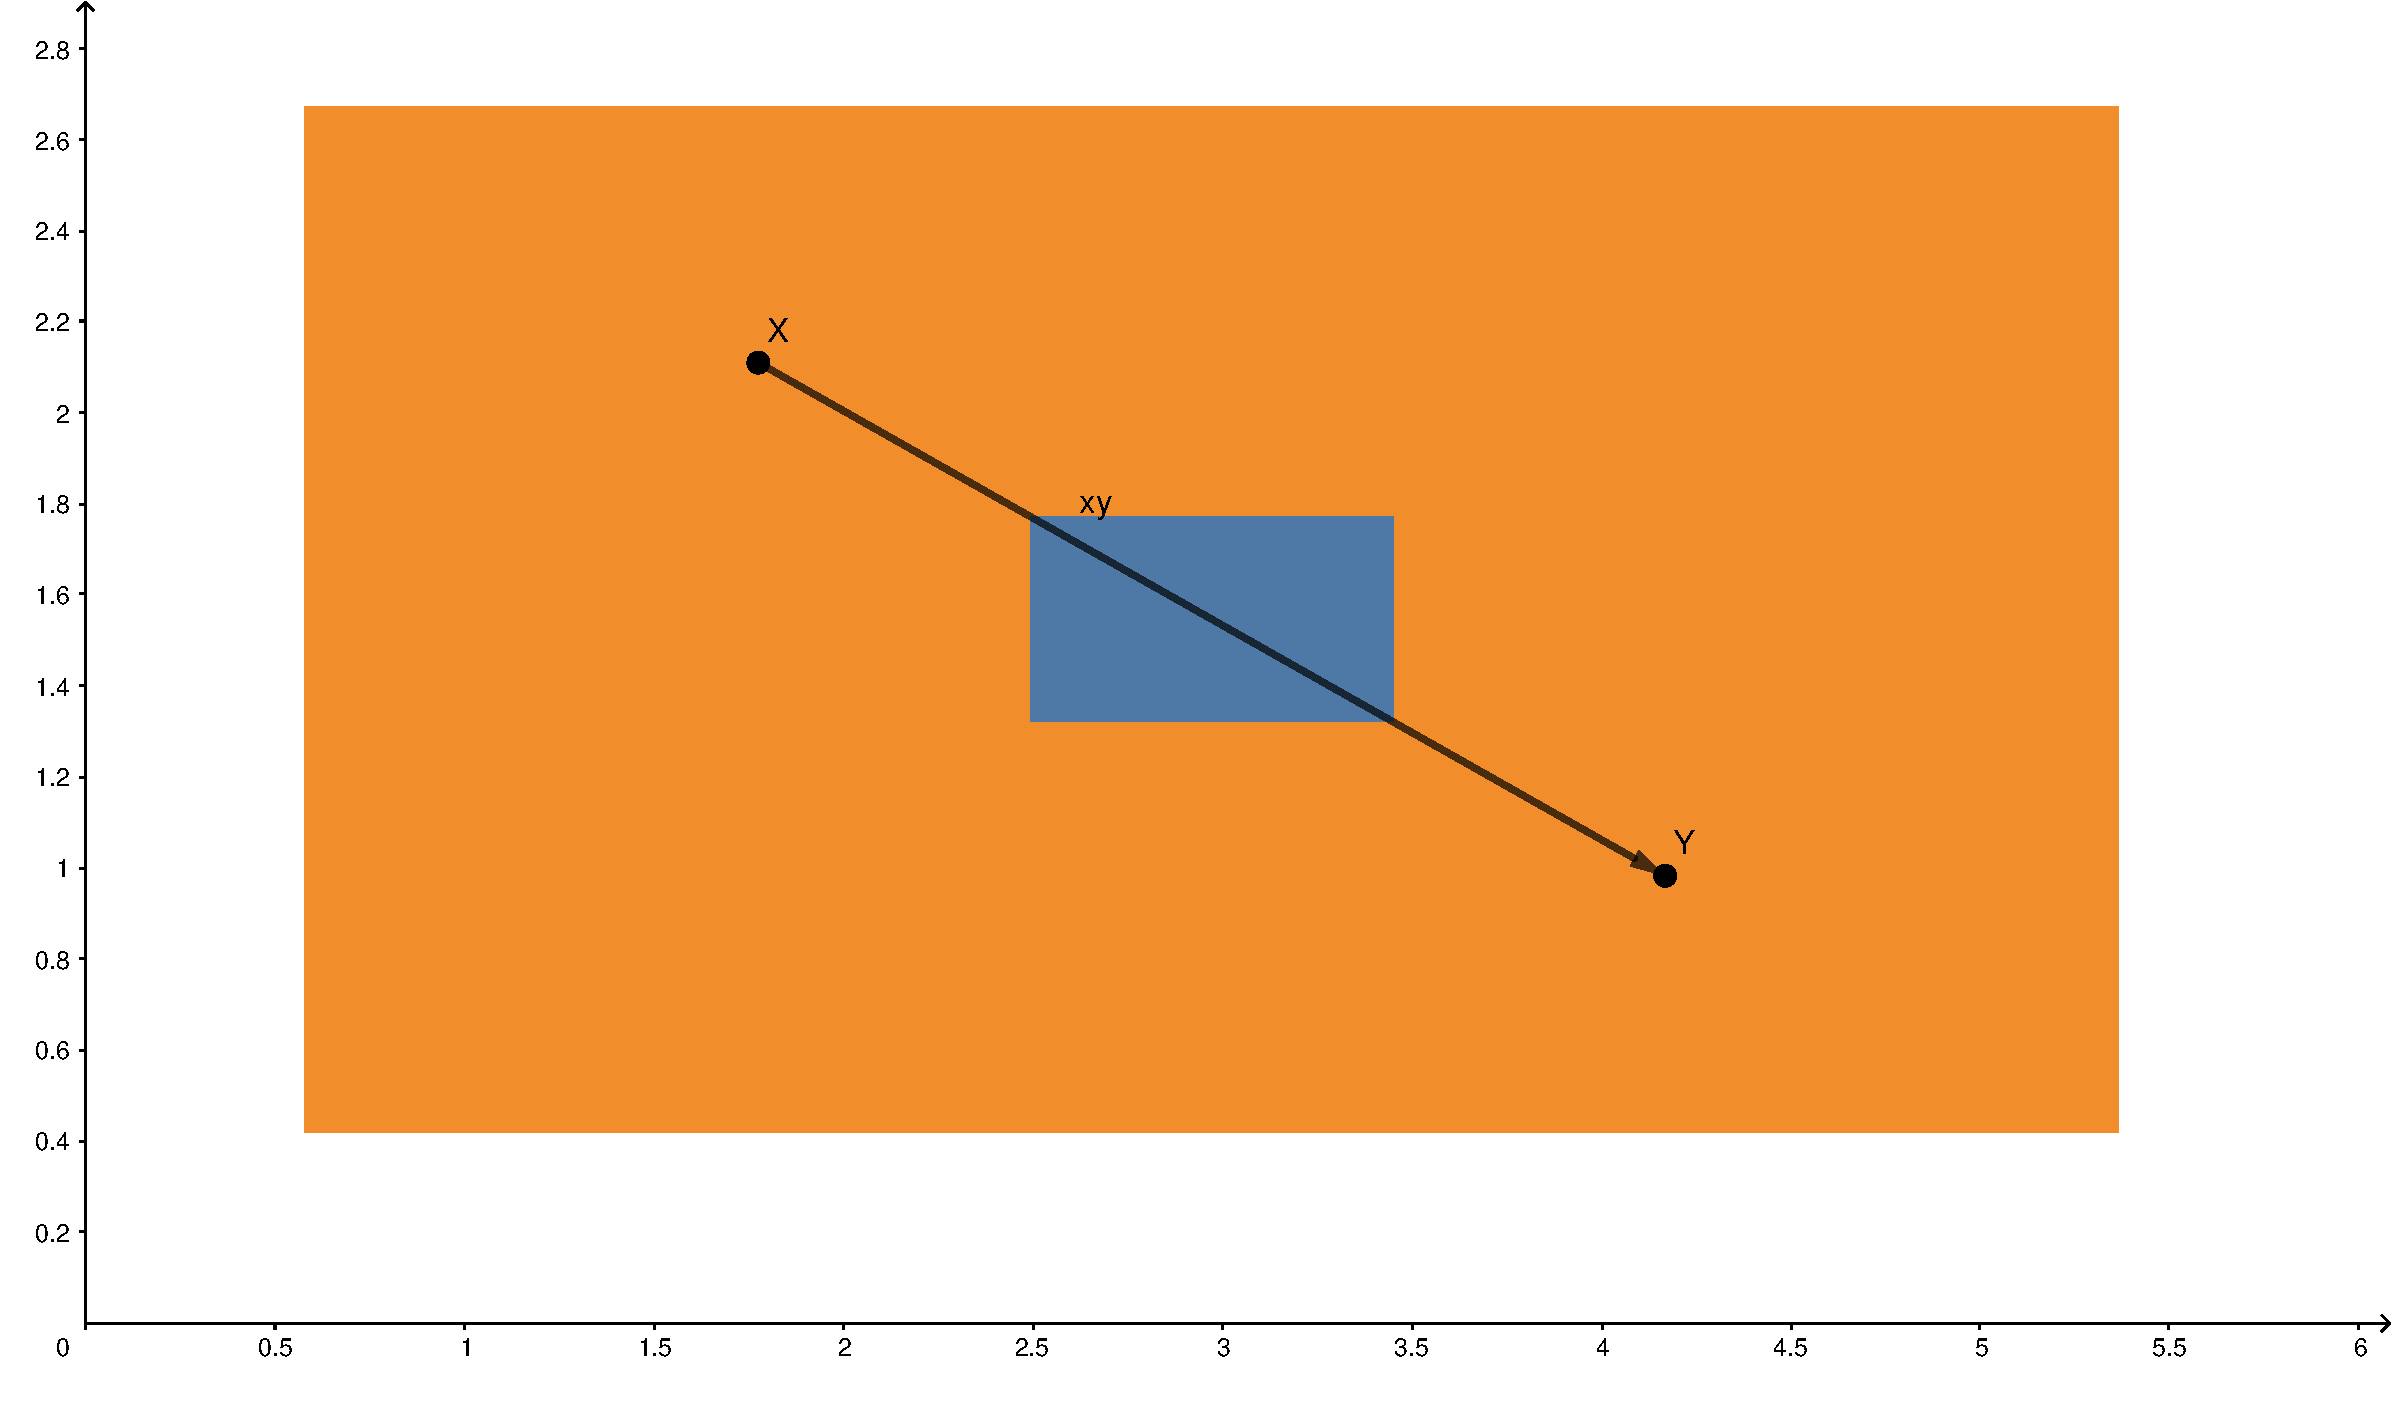
\includegraphics[width=\textwidth]{img/BLX.pdf}
        \caption{Blend crossover sample space with $\alpha=0.5$ (orange) and $\alpha=-0.3$ (blue) in two dimensions.}
        \label{fig:blendcrossoverexample}
    \end{subfigure}
    \hfill
    \begin{subfigure}[t]{0.45\textwidth}
        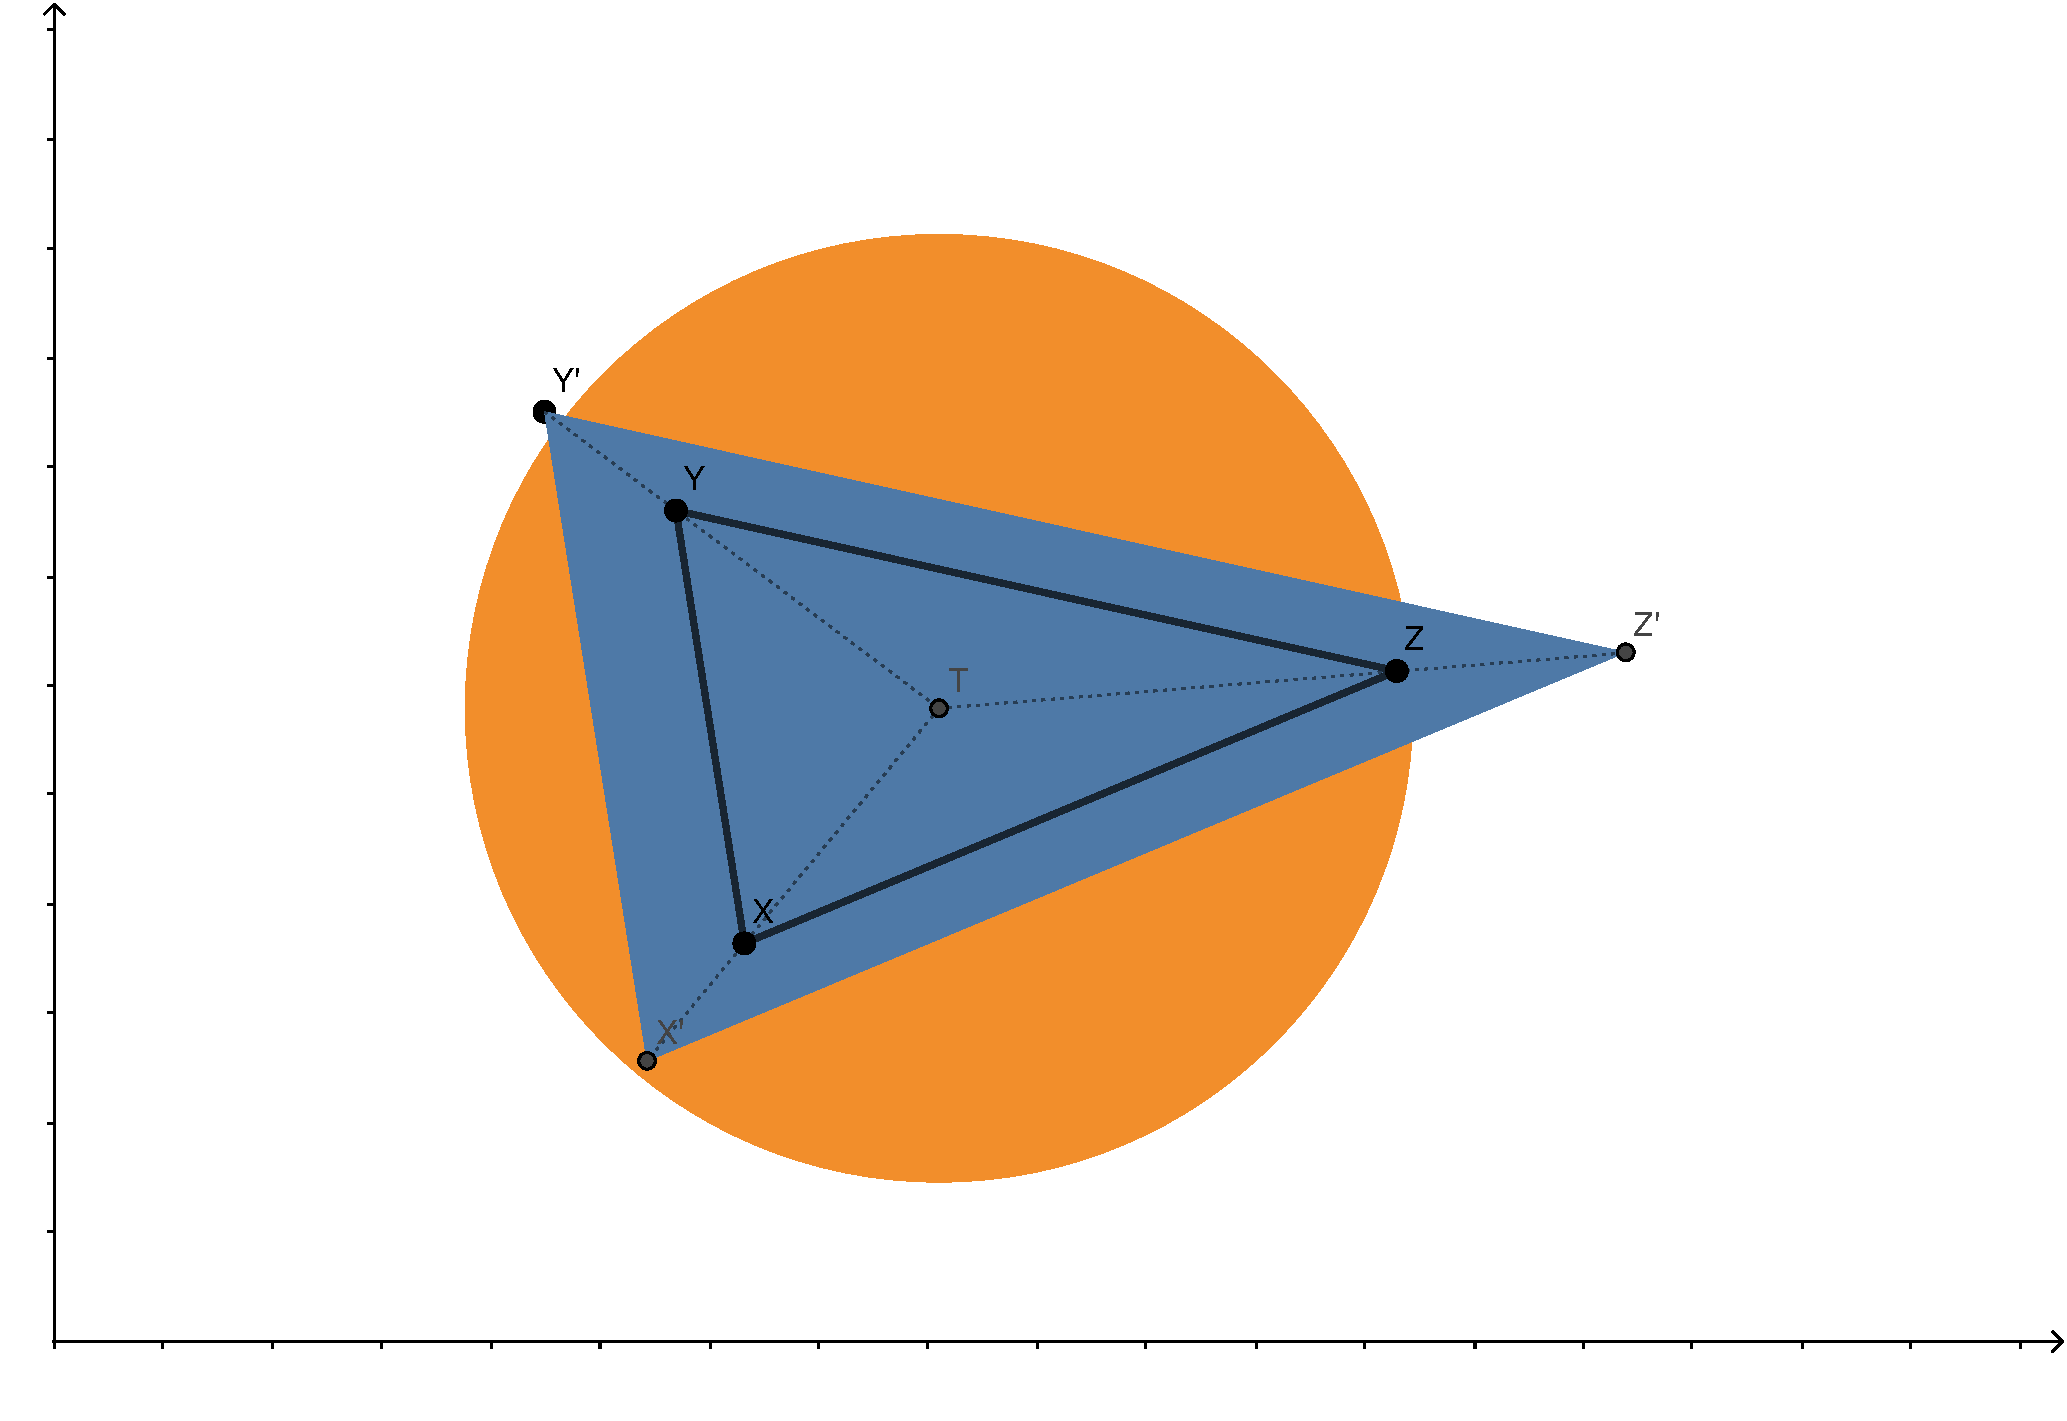
\includegraphics[width=\textwidth]{img/SimplexCrossover.pdf}
        \caption{Simplex crossover example in two dimensions. Sampling space of simplex (blue) and hypersphere (orange).}
        \label{fig:simplexcrossoverexample}
    \end{subfigure}
    \caption{\acrshort*{acc:es} crossover operators}
\end{figure}

Another type of crossover operator is \emph{simplex crossover}\index{crossover \acrshort*{acc:es}!simplex}. It uses simplex to sample sample offsprings. Simplex is a generalization of triangle into more dimensions. It is defined in $n$--dimensional space using $n+1$ points. For two dimensional space is simplex triangle, for three dimensional space is simplex tetrahydron and so on. From the definition, the simplex crossover require $n+1$ parents $\mathbf{p_1}, \mathbf{p_2}, \dots, \mathbf{p_n}, \mathbf{p_{n+1}}$. It calculate their centroid
$$
\mathbf{k}=\frac{\sum_{i=1}^{n+1} \mathbf{p_i}}{n+1}
$$
and then expand the simplex by $\varepsilon$ along each of the direction $\mathbf{p_k} - \mathbf{k}$. As a result, this new, expanded, simplex is defined by the points
\boldmath
$$
p'_i = p_i + \varepsilon\left( p_i - k \right).
$$
\unboldmath
From this simplex, the offspring are sampled. Example of simplex in two dimensional space is in the figure \ref{fig:simplexcrossoverexample} with $\varepsilon=1.5$.
I would argue, that the hypersphere sample space can be used as well, as is shown in figure \ref{fig:simplexcrossoverexample} as well with $\varepsilon=1.2$.
% TODO not implemented
% In the Introduction to Evolutionary Algorithms, another types of crossovers like Simulated Binary Crossover and Unimodal Normal Distribution Crossover are described as well. I can discuss them when they become relevant.

%%%%%%%%%%%%%%%%%%%%
%%%%  MUTATION  %%%%
%%%%%%%%%%%%%%%%%%%%
\subsection{\texorpdfstring{\acrshort*{acc:es} mutation operators}{}}

Equivalent of bit--flip mutation in \acrshort{acc:ga} is \emph{uniform mutation}\index{mutation \acrshort*{acc:es}!uniform}. It replaces gene by random value sampled from $U(l,u)$ with small probability $p_m$, where interval $\left[l,u\right]$ is the domain of the scalar. This operator basically tries random numbers and can rarely lead to good solution. Moreover, it does not exploit distribution of the population.
% TODO check whether is implemented

More successful and frequently used is \emph{normal mutation}\index{mutation \acrshort*{acc:es}!normal}. It performs small change of the individual by adding sample from normal distribution with zero mean to each gene.
$$
p_i = p_i + N(0,\sigma)
$$
The $\sigma$ is mutation strength parameter and is usually kept low. Notice that normal mutation does not use mutation probability $p_m$. Because the $\sigma$ is usually small and the distribution has zero mean, the changes does not influence the population too much.

Normal mutation can be further extended to adapt to more complicated problems. Instead of $\sigma$ variable, it is possible to introduce $\boldsymbol{\sigma}$ vector, that allows different deviation in each dimension.
$$
p_i = p_i + N(0,\sigma_i)
$$ 
To address non--separable functions, we may need the whole covariance matrix $\Sigma^{n \times n}$ for successful adaptation. Normal mutation with covariance matrix is sometimes called correlated mutation. Notice that in order to use correlated mutation in $n$ dimensions, the algorithm needs $\frac{n\left(n+1\right)}{2}$ parameters just for the correlation matrix and therefore correlated mutation has just a small practical usage on its own. Another algorithms addressed this issue -- probably the best well--known is the \acrfull{acc:cma}.

Normal distribution is probably the most used mutation distribution, but other distributions are possible as well. \citet*{CauchyDistributionMutation} used Cauchy distribution to faster the search. As shown in figure \ref{fig:mutationdistributionnormalcacuchy}, Cauchy distribution does not  decrease as fast as normal distribution and therefore search bigger genotype space. On the other hand, if we desire to shrink the searching space, we may use polynomial distribution, which probability density function is defined as
$$
p(x)=0.5 \left(n + 1\right)\left( 1 - \abs{x} \right)^n
$$ 
where $n$ user--defined parameter and function domain is interval $\left[-1,1\right]$. Example of polynomial distribution is in figure \ref{fig:mutationdistributionpolynomial}.

\begin{figure}
    \begin{subfigure}[t]{0.45\textwidth}
        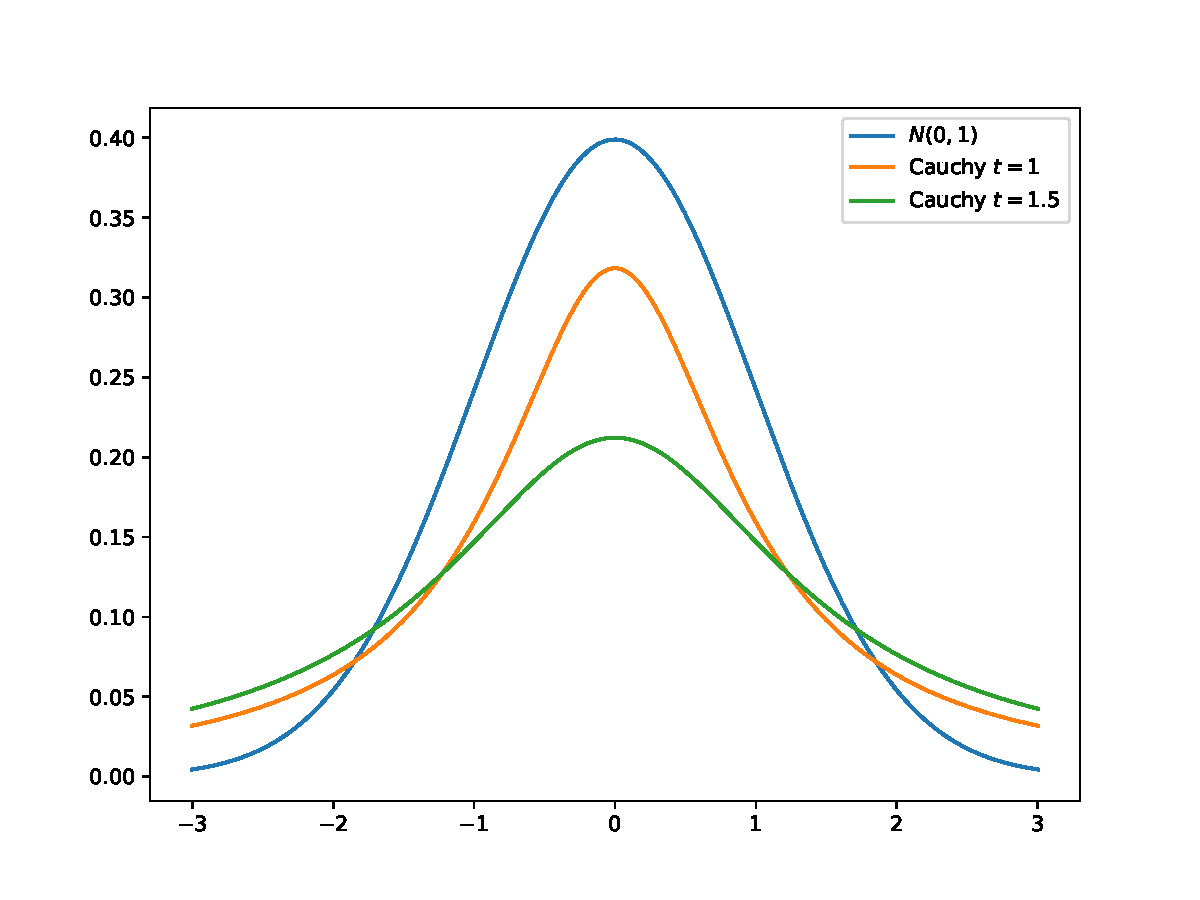
\includegraphics[width=\textwidth]{img/render_distributions_normalcauchy.pdf}
        \caption{Normal and Cauchy distributions.}
        \label{fig:mutationdistributionnormalcacuchy}
    \end{subfigure}
    \hfill
    \begin{subfigure}[t]{0.45\textwidth}
        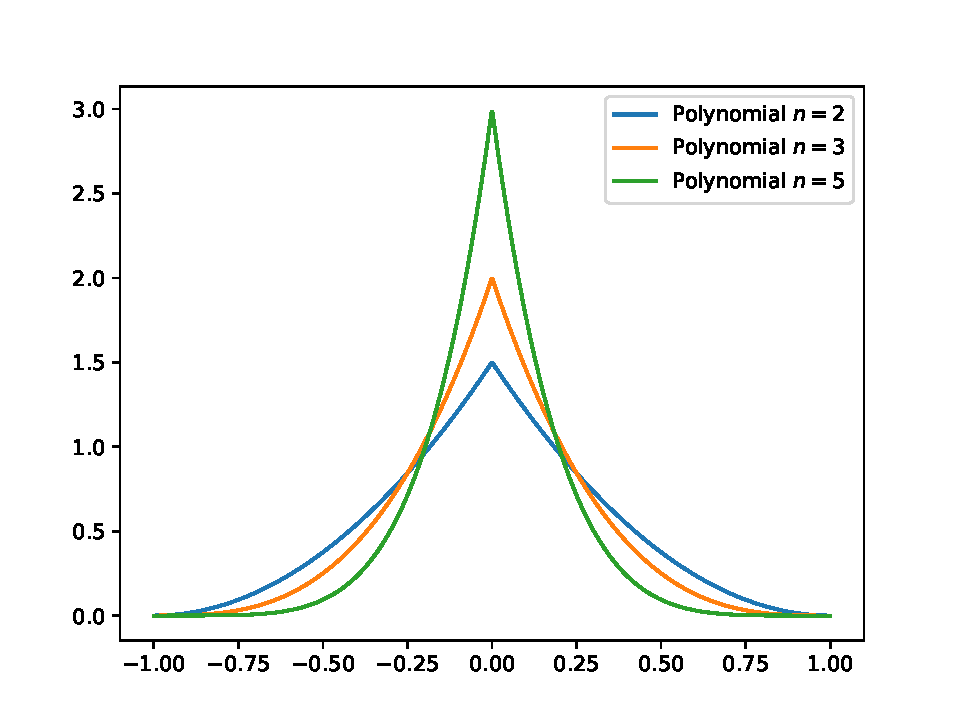
\includegraphics[width=\textwidth]{img/render_distributions_polynomial.pdf}
        \caption{Polynomial distributions.}
        \label{fig:mutationdistributionpolynomial}
    \end{subfigure}
    \caption{Mutation distributions}
\end{figure}


%%%%%%%%%%%%%%%%%%%%%%
%%%%  ADAPTATION  %%%%
%%%%%%%%%%%%%%%%%%%%%%
\subsection{Adaptive operators}

%%%%%%%%%%%%%%%%%%%%%%%%%%%%%%%%%%
%%%%  DIFFERENTIAL EVOLUTION  %%%%
%%%%%%%%%%%%%%%%%%%%%%%%%%%%%%%%%%
\subsection{Differential evolution}
